\label{sec:optimizers}










We now motivate specific instantiations of optimizer algorithms composed of the algorithmic strategies outlined in Section~\ref{sec:design}. %
We describe the algorithms that are the focus of our experimental investigation, and leave 
full descriptions for the remaining optimizers to Appendix~\ref{sec:algo_appendix}.


\subsection{Bootstrap Random Search}

\begin{figure}[H]
    \centering
    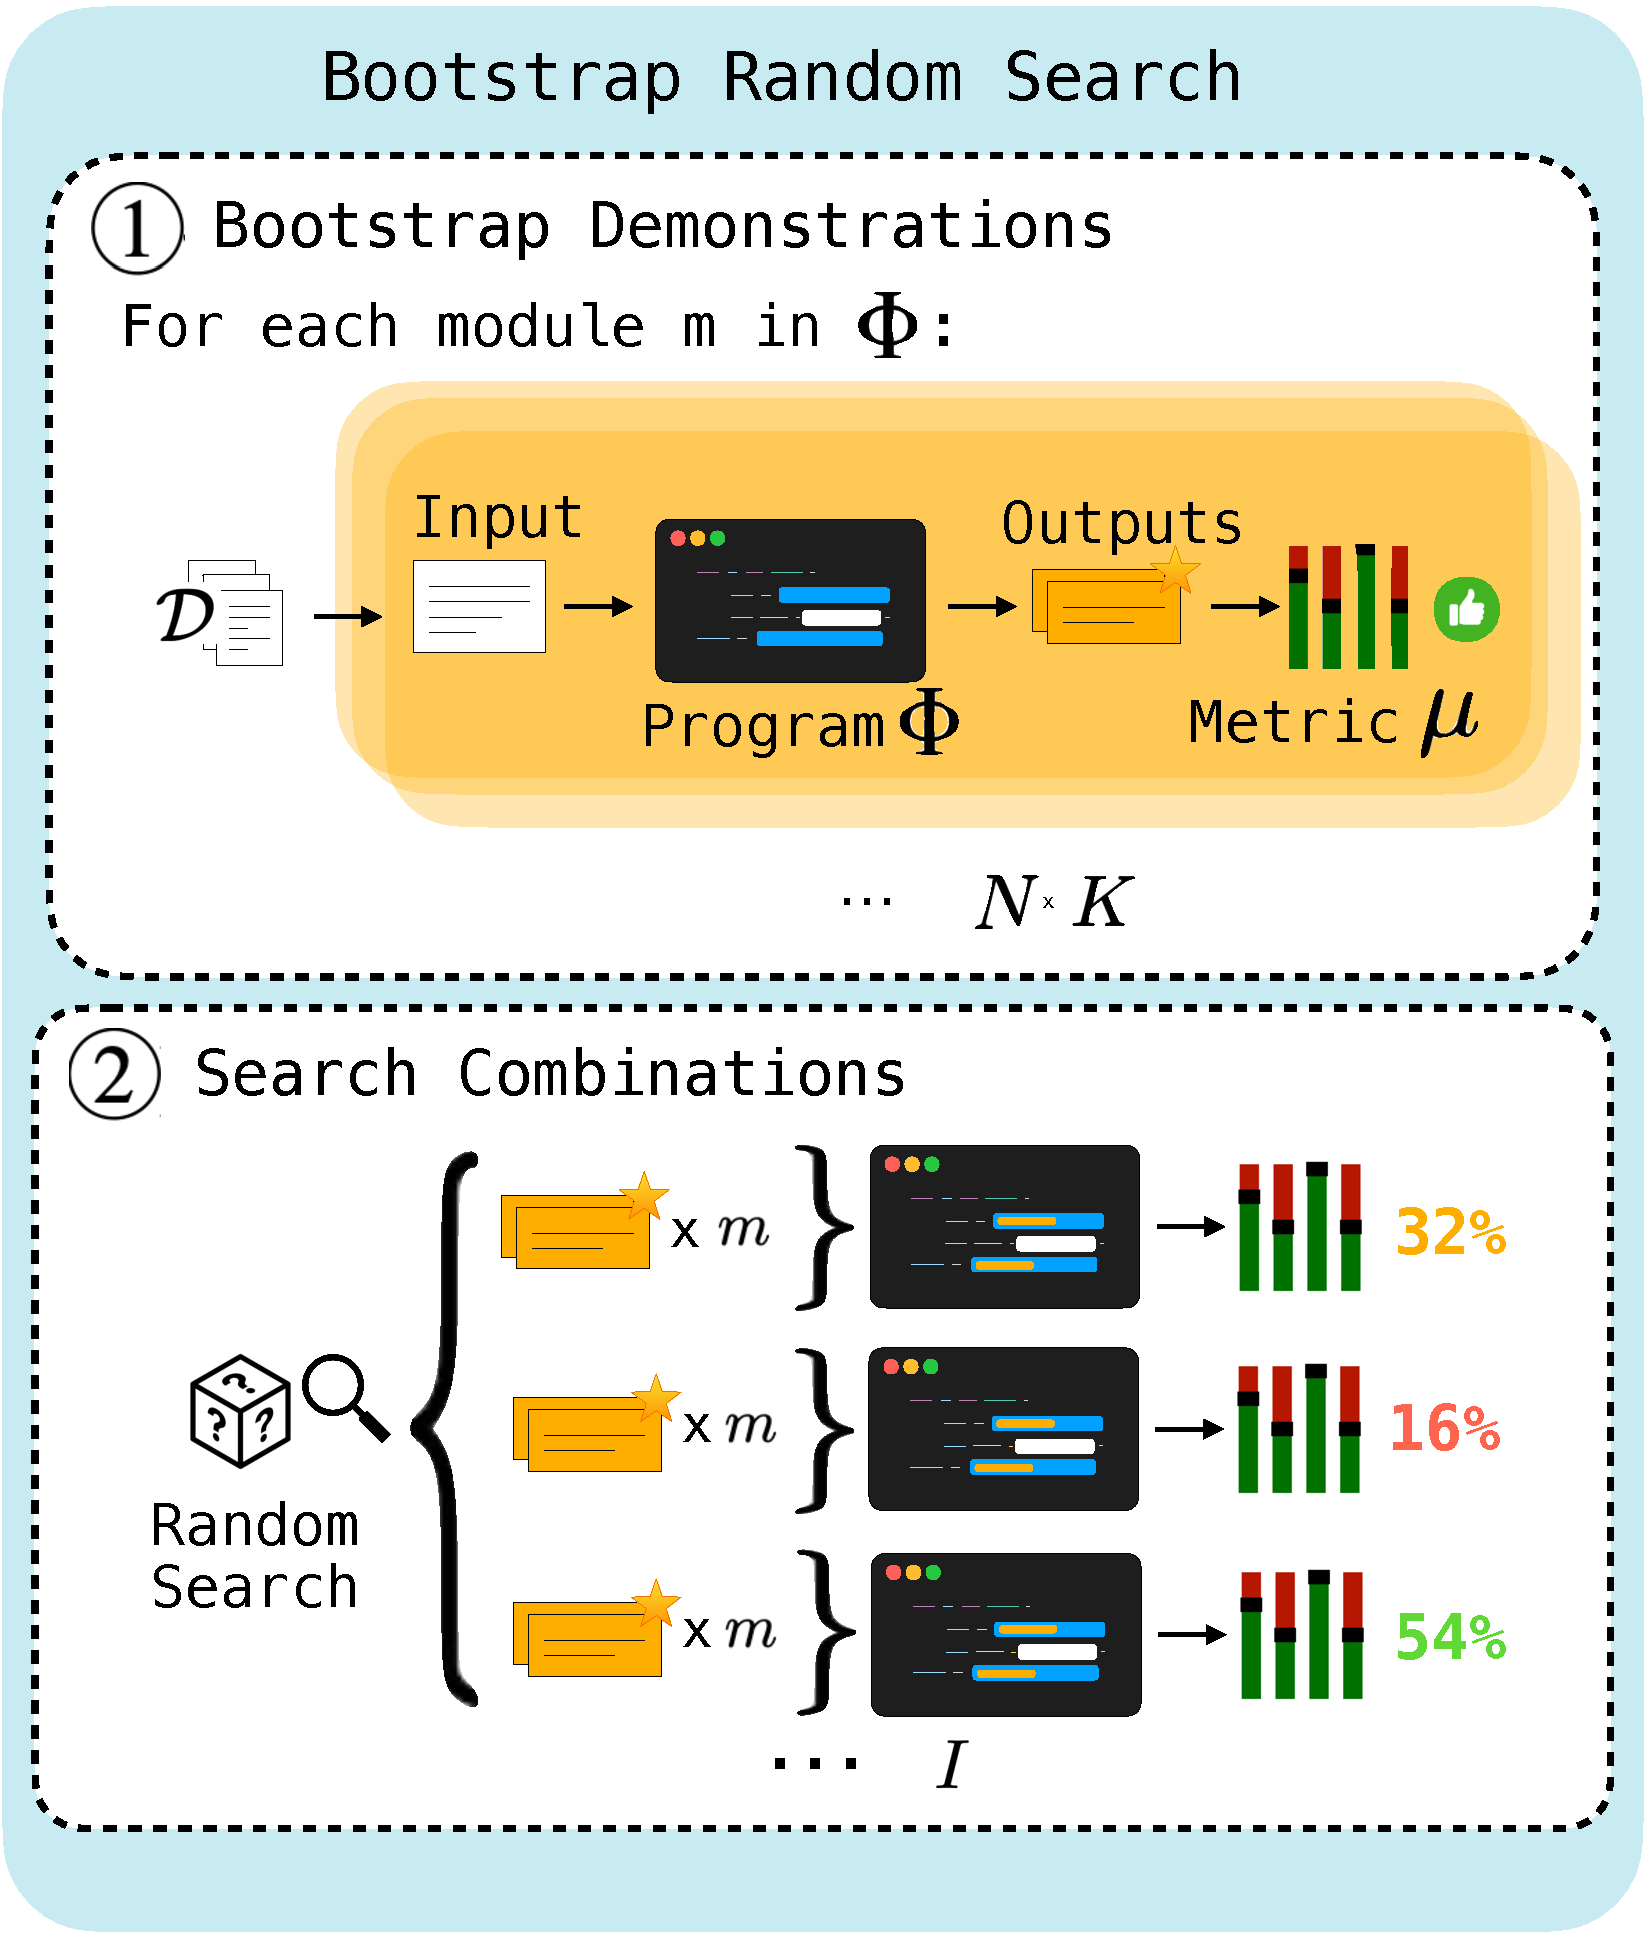
\includegraphics[width=0.96\linewidth]{figures/bootstrap_vertical.pdf}
    \caption{Bootstrap Random Search. In Step 1, demonstrations are bootstrapped by running training inputs through the program $\Phi$ and keeping traces that produce sufficiently high scoring outputs, as judged by metric $\mu$. In Step 2, these bootstrapped demonstration sets are searched over using random search, and the most performant set is returned.}
    \label{fig:bs_figure}
\end{figure}

\citet{khattab2024dspy} achieve strong results by generating and selecting task demonstrations for each module using random search. This approach fits into our general framework and serves as a strong baseline in our experiments. This optimization procedure (highlighted in Figure \ref{fig:bs_figure}) works as follows:


The hyperparameters include: $K$, the number of demonstrations to use for each module in $\Phi$, and $N$, the number of total sets to bootstrap and evaluate.
To \textbf{Initialize}, $N$ sets of few-shot examples are bootstrapped using the Bootstrapping Demonstrations procedure described in \ref{sec:prompt_proposal}. An input-output pair $(x, x') \in \mathcal{D}$ is randomly sampled from $\mathcal{D}$, where $x$ is an input to the program and $x'$ contains metadata (e.g.\ empty or final answers). Then, $\Phi(x)$ is run, which generates a full trace $\tau$ of the steps that $\Phi$ used for example $x$. If the output scores highly, i.e.\ $\mu(\Phi(x), x') \geq \lambda$ for some threshold $\lambda$ and given metadata or final label $x'$, we assume the trace to be correct, and use the inputs / outputs for each module in the trace as candidate few-shot examples. This process is repeated until $N$ sets of $K$ few-shot examples for each module have been bootstrapped.
To \textbf{Propose}, we sample a set of few-shot examples and use them to parameterize each module in $\Phi$.
To \textbf{Update}, the parameterized $\Phi$ is added to a global store along with its evaluation score on the training set (or a dedicated validation split thereof).
To \textbf{ExtractOptimizedSets}, the top-scoring assignment is returned.


\subsection{Module-Level OPRO}

\begin{figure}[H]
    \centering
    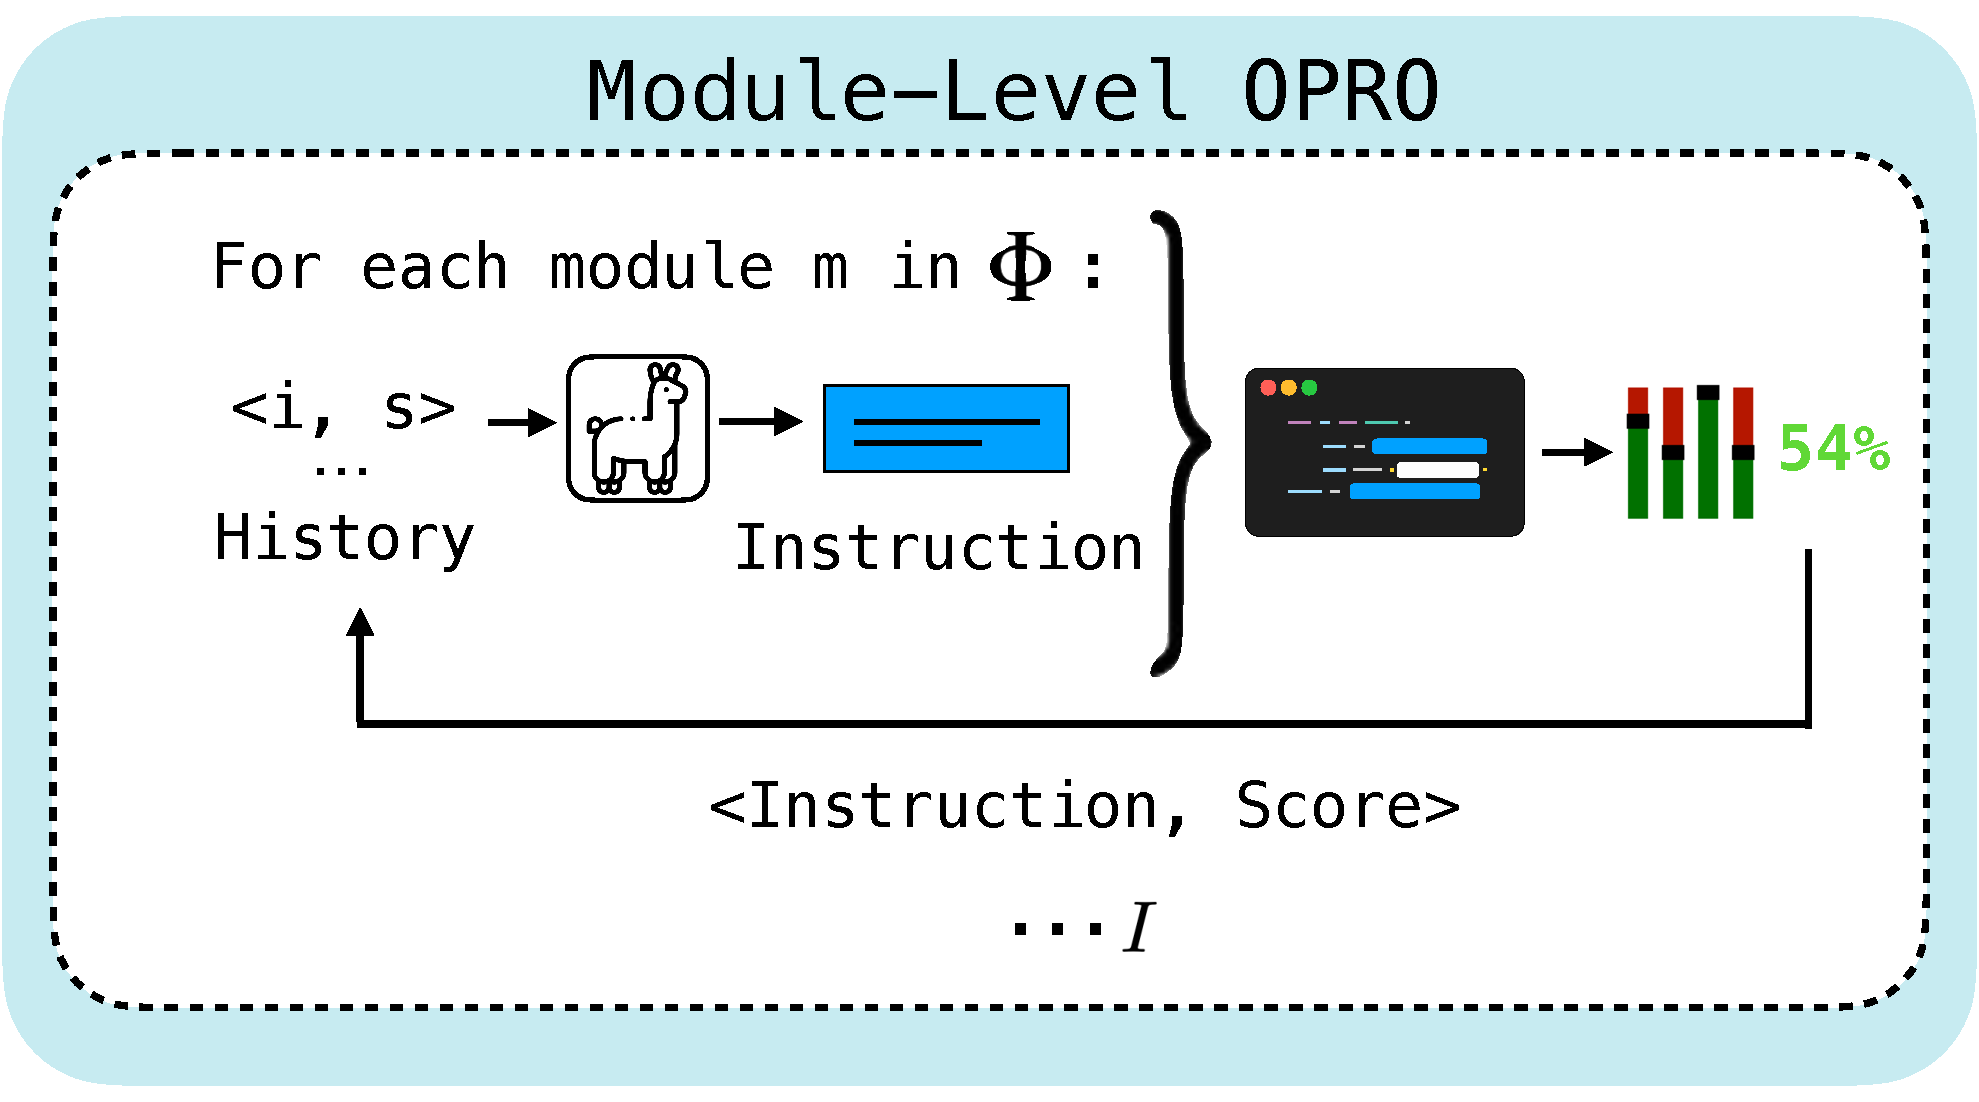
\includegraphics[width=0.95\linewidth]{figures/module_level_opro.pdf}
        \caption{The Module-Level OPRO optimizer. A history of module-level instructions and program score pairs are given as input to the proposer LM to generate a new instruction for each module. These are then evaluated in the program, and the resulting score is added back with each module's instruction to the module's history. The process repeats for $I$ iterations.}
    \label{fig:opro_figure}
\end{figure}

We seek to extend the OPRO algorithm \citep{yang2023large} to an arbitrary LM program $\Phi$, e.g.\ with $m \geq 1$ stages embedded in a larger program. In OPRO, the proposer LM is provided with a history of proposed instructions and their scores, allowing it to learn to propose better instructions over time. To extend OPRO, we first consider an approach we refer to as Module-Level OPRO, in which we assume that the program score is a good enough proxy for an individual instruction's quality. In other words, even though the program is parameterized with $m$ instructions, we will assume that the score is reflective enough of each. Module-level OPRO (Figure \ref{fig:opro_figure}) works as follows: 

To \textbf{Initialize}, a seed instruction is used to parameterize each module in $\Phi$, which is evaluated. To \textbf{Propose}, the resulting score and the $i_{th}$ module's instruction are inputted into the proposer LM to create a new instruction for module $i$. This is done for all $m$ modules. The set of $m$ generated instructions are then used to parameterize $\Phi$, and the parameterized program is evaluated. To \textbf{Update}, each instruction and the score is added to the history for each module. The OPRO sub-routine is run again with the updated histories to create a new set of instructions. We note that optimizers for each stage are provided with histories of module-level trajectories and proxy scores only. This process continues until the maximum number of iterations is reached. To \textbf{Extract\-OptimizedSets}, the parameterization of $\Phi$ that scored highest is returned.







\subsection{MIPRO}
\label{mipro_section}

\begin{figure}[H]
    \centering
    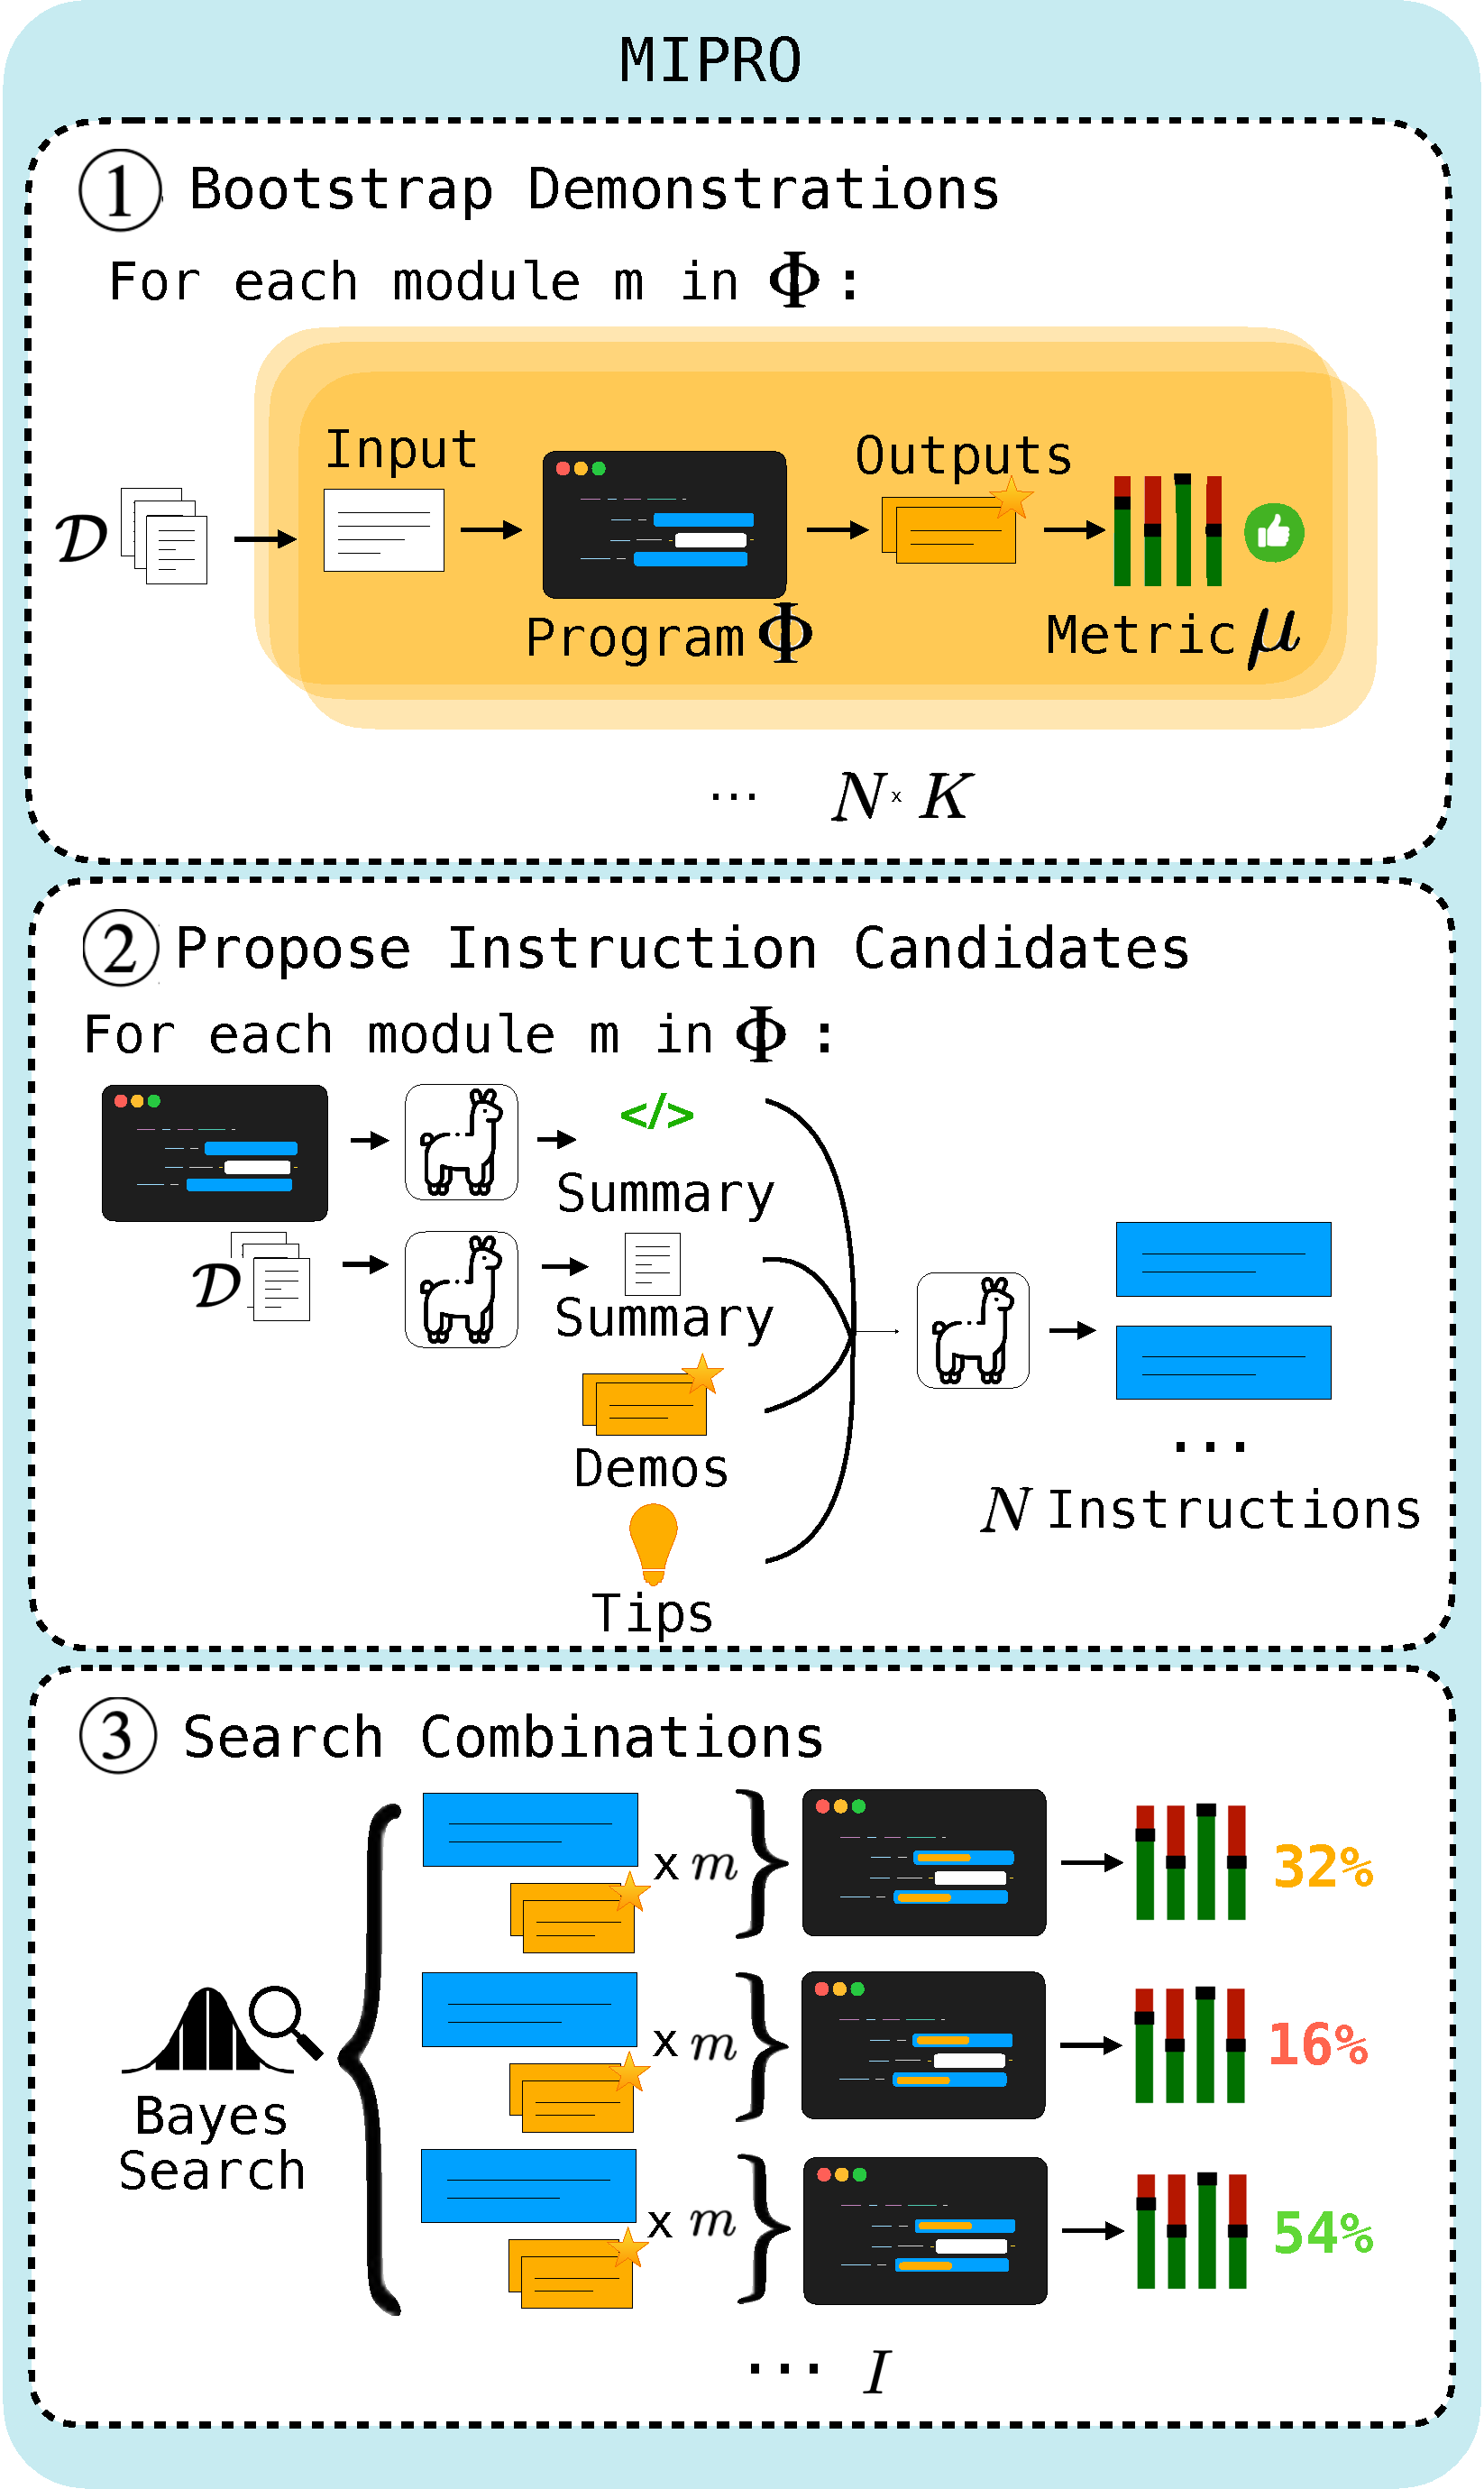
\includegraphics[width=0.97\linewidth]{figures/mipro_vertical.pdf}
        \caption{The MIPRO optimizer. In Step 1, demonstrations are bootstrapped using the same process from Step 1 of Bootstrap Random Search. In Step 2, instructions are proposed using the grounding strategy described in \ref{sec:prompt_proposal}. In Step 3, Bayesian optimization is used to find the best performing combination of instruction and demonstration candidates.}
    \label{fig:MIPRO_figure}
\end{figure}
To relax OPRO's strong assumptions, we propose the use of a Bayesian surrogate model to explicitly learn the sensitivity of task-level scores to module-level parameters such as instructions and demonstrations throughout optimization. We refer to this approach as MIPRO (\underline{M}ulti-prompt \underline{I}nstruction \underline{PR}oposal \underline{O}ptimizer). By separating the task of credit assignment from prompt proposal, we allow for the proposal LM to focus on the task of proposal only. Credit assignment and final selection is then done post-hoc using our surrogate model.

Bayesian optimization is known for its robustness to noise, as it effectively incorporates uncertainty into the optimization process \cite{snoek2012practical}. We therefore propose evaluating over mini-batches of our training data, rather than the full set with each iteration. This allows us to explore and exploit parameter configurations more efficiently. The MIPRO algorithm (Figure \ref{fig:MIPRO_figure}) is as follows:

To \textbf{Initialize}, MIPRO bootstraps a set of $N$ few-shot example sets and instructions per module using the Bootstrap Demonstration and Grounding strategies respectively, found in \ref{sec:prompt_proposal}. Latent categorical variables representing the choice of few-shot examples and instructions for each module are initialized with a uniform prior. To \textbf{Propose}, we use the sampling rule from the Tree-structured Parzen Estimator \citep{bergstra2011algorithms} to select the instructions and few-shot examples used to parameterize $\Phi$. To \textbf{Update}, this parameterized $\Phi$ is scored on a randomly selected mini-batch of B samples, and the scores are used to update the Estimator's priors over parameter quality. To \textbf{ExtractOptimizedSets}, every $S$ steps, the candidate parameterizations of $\Phi$ with the highest mean score over trials is evaluated on the full train-set. At the end, the highest scoring fully evaluated parameterization is returned as the optimal assignment.






\subsection{Other MIPRO variants}


\hspace*{\parindent}
\textbf{0-Shot MIPRO} is a straightforward extension of MIPRO that simply optimizes over instructions only, rather than both jointly. This could be desirable for cost or context-window constraints.

\textbf{Bayesian Bootstrap} is the restricted version of MIPRO to optimizing over bootstrapped demonstrations. This may be ideal when few-shot examples are essential to the task or when we have already identified a good instruction and want to use our budget to optimize demos alone.

\textbf{MIPRO++} applies a Bayesian surrogate model to optimize \textit{proposal} hyperparameters, rather than the choice of LM program parameters themselves. This follows directly from the Learning to Propose strategy discussed in Section~\ref{sec:prompt_proposal}. In the full form of this approach, a surrogate  model is used to learn optimized parameters for proposing instructions, as well as for bootstrapping demonstrations. However, in the context of this work, we focus on evaluating this approach for optimizing our instruction proposal strategy specifically (described next). 

\textbf{0-Shot MIPRO++} tunes instructions by meta-optimizing how or whether our Grounded instruction proposal strategy uses the dataset summary (\texttt{boolean}), uses the program summary (\texttt{boolean}), adjusts the proposer LM temperature (\texttt{float}), provides the proposer LM a plain-text tip on prompt engineering  (\texttt{categorical}; see Appendix~\ref{sec:grounding_details}), and selects a specific set of bootstrapped demos to show to the proposer LM (\texttt{categorical}). A Bayesian model with the same mini-batching strategy employed in MIPRO is then used to optimize over these hyperparameters. A program with the newly proposed instruction is evaluated on each trial, using the mini-batching approach described earlier. The best fully-evaluated program is returned.


\begin{table*}[tp]
\begin{center}
\resizebox{\textwidth}{!}{%
\begin{tabular}{lllccl}
\toprule
\textbf{Benchmark} & \textbf{Task Type} & \textbf{Program} & \textbf{Modules} & \textbf{LM Calls} & \textbf{Metric} \\ \midrule
HotPotQA & Multi-Hop QA & Multi-Hop Retrieval & 2 & 3 & Exact Match \\
HotPotQA Conditional & Multi-Hop QA & Multi-Hop Retrieval & 2 & 3 & Custom \\
Iris & Classification & Chain of Thought & 1 & 1 & Accuracy \\
Iris-Typo & Classification & Chain of Thought & 1 & 1 & Accuracy \\
Heart Disease & Classification & Answer Ensemble & 2 & 4 & Accuracy \\
ScoNe & Natural Language Inference & Chain of Thought & 1 & 1 & Exact Match \\
HoVer & Multi-Hop Claim Verify & Multi-Hop Retrieval & 4 & 4 & Recall@21 \\
\bottomrule
\end{tabular}
}
\caption{DSPy Optimizer Benchmark and associated programs. We benchmark our optimizers on seven diverse programs. Additional details are in Appendices~\ref{sec:task_desc} and~\ref{sec:lm-program-appendix}.}
\label{tab:optimizer-benchmark}
\end{center}
\end{table*}

\subsection{Other OPRO variants}

\hspace*{\parindent}
\textbf{Program-Level OPRO} provides the proposer LM with a history of \textit{full, multi-stage} trajectories and relies on it to assign credit for task-level scores to the program stages. While Module-level OPRO embeds the assumptions that there is no inter-assignment dependency and that credit assignment across modules is equal, Program-level OPRO assumes that an LM will successfully complete credit-assignment when provided with long trajectory histories. These are all very strong assumptions. In particular, information contained in histories is likely to be lost as history length grows \cite{liang_litm}. In our experiments, we opt for using Module-level OPRO because Program-Level OPRO is more complex and did not appear to provide additional performance gains.

\textbf{CA-OPRO} ``Coordinate-Ascent'' OPRO (CA-OPRO) employs a greedy credit assignment approach to extend OPRO to multi-stage settings. It iterates through each module $m$ in the program, proposes a new set of $N$ instructions for $m$ using Module-Level OPRO's proposal function, and evaluates each proposal by keeping all other parameters in the program fixed. It then updates module $m$ with the best evaluated instruction so far, and repeats with the next module. This entire process is then repeated $D$ times. From initial experiments, we found CA-OPRO's performance did not justify its inefficiency, so we focus our experiments on evaluating other methods more thoroughly.
